\newpage
\section{Valutazione dei dataset}
Durante la ricerca per trovare dei dataset utilizzabili per l'addestramento del modello
oltre a quelli messi a disposizione dell'azienda si è trovato il dataset 
\cite{guillem_montalban_faet_2025_17866344} che tuttavia non contiene il canale SWIR ed è stato effettuato da un drone e non da un satellite.
Per valutare la bontà dei dati e se un ipotetico classificatore è in grado di distinguere i vari pixel si è andati a plottare i valori delle bande.
Si mostrano di seguito i plot.
Nello specifico si sono create delle bbox di diverse tipologie:
\begin{itemize}
    \item bbox per indicare le non piante
    \item bbox per indicare le piante avocado
    \item bbox per indicare le piante di un'altra tipologia (1)
    \item bbox per indicare le piante di un'altra tipologia (2)
\end{itemize}
Le bbox (Bounding Box) sono riquadri di ritaglio nell'immagine su cui si andrà a lavorare.
Per ogni bbox di una tipologia si fa il plot dei pixel contenuti all'interno della bbox. 
Di seguito si mostrano i plot per quanto riguarda le bbox non piante e le bbox
che contengono le piante avocado \ref{fig:plotavocadoRGB}

%inizio dei plot
\begin{figure}[htbp]
    \centering
    \begin{minipage}{0.30\textwidth}
    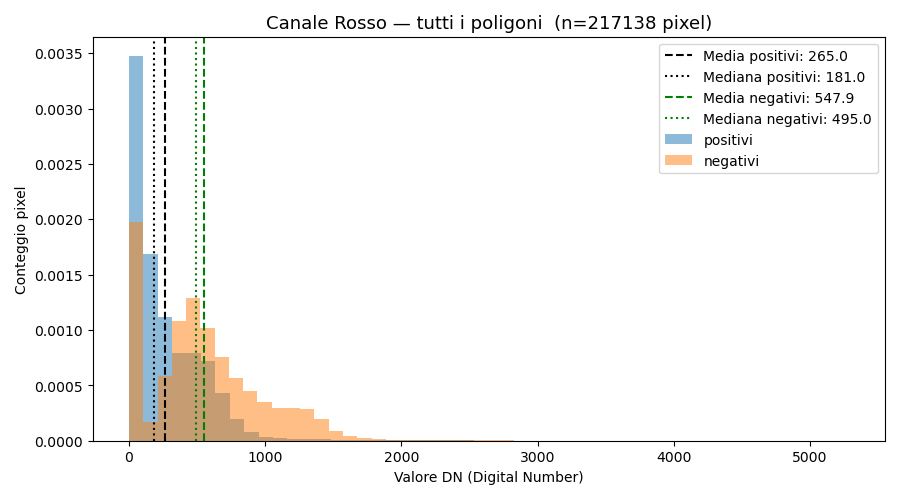
\includegraphics[width=0.9\textwidth]{capitoli/capitolo2/images/avocado/Satelliterosso.png}
    \end{minipage}
    \hfil 
    \begin{minipage}{0.30\textwidth}
    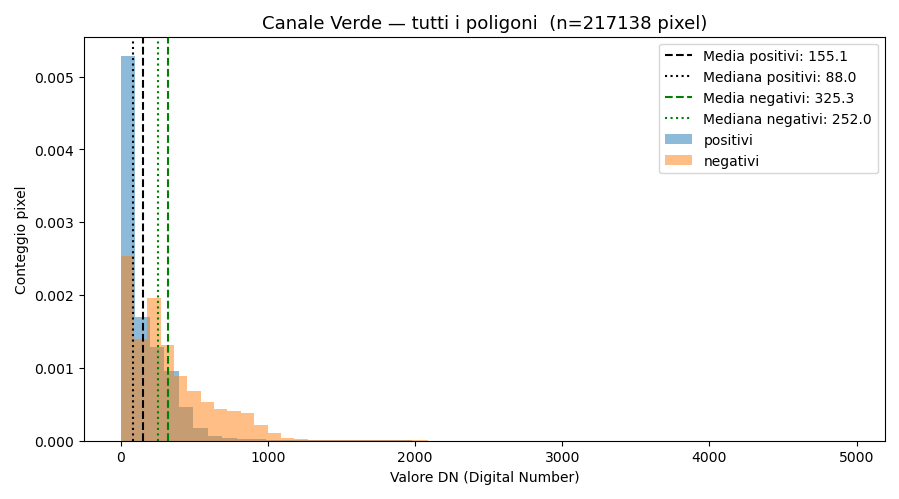
\includegraphics[width=0.9\textwidth]{capitoli/capitolo2/images/avocado/Satelliteverde.png}
    \end{minipage}
    \hfil
    \begin{minipage}{0.30\textwidth}
    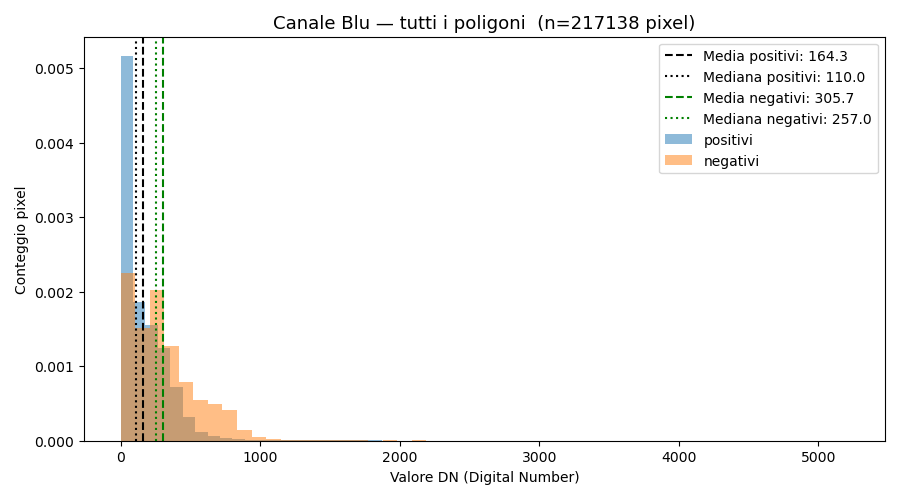
\includegraphics[width=0.9\textwidth]{capitoli/capitolo2/images/avocado/Satelliteblu.png}
    \end{minipage}
    \caption{Si mostrano i grafici RGB delle bbox degli avocado e dei non pianta}
    \label{fig:plotavocadoRGB}
\end{figure}

Di seguito si mostrano i plot delle bande dell'infrarosso (RedEdge, NIR, SWIR) \ref{fig:plotavocadoInfrarosso}:
\begin{figure}[htbp]
    \centering
    \begin{minipage}{0.30\textwidth}
    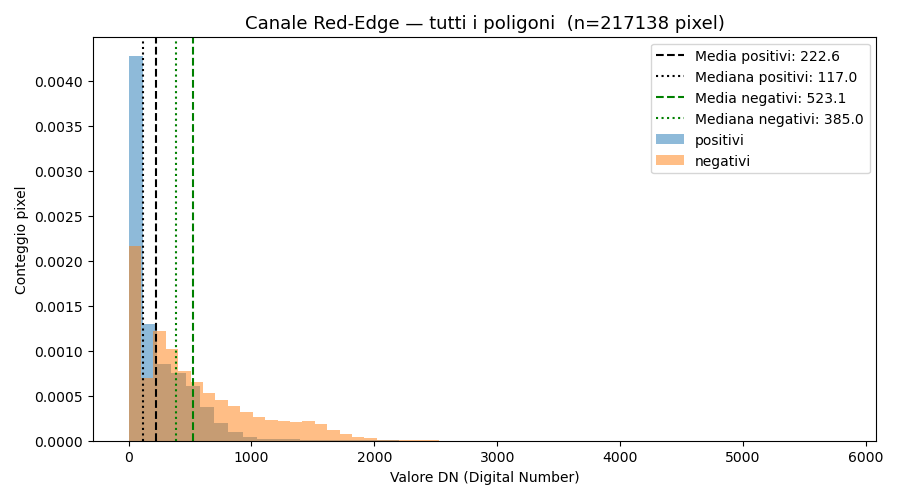
\includegraphics[width=0.9\textwidth]{capitoli/capitolo2/images/avocado/SatelliteRedEdge.png}
    \end{minipage}
    \hfil 
    \begin{minipage}{0.30\textwidth}
    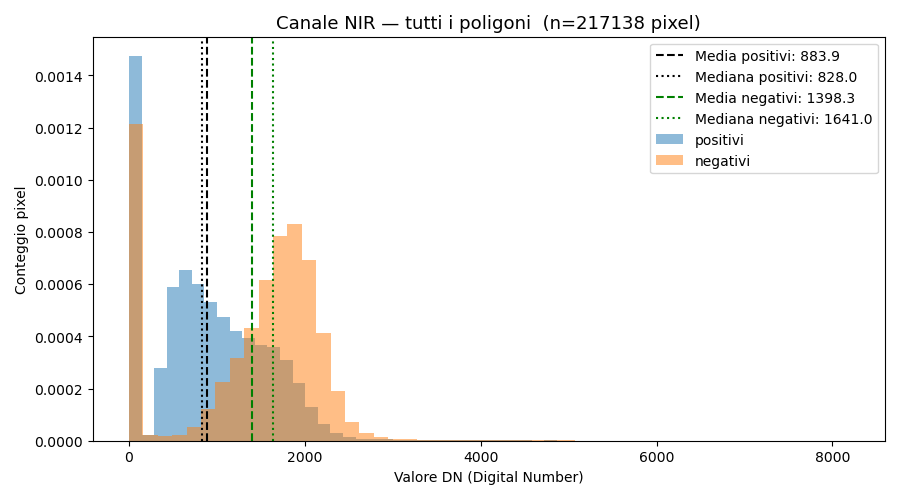
\includegraphics[width=0.9\textwidth]{capitoli/capitolo2/images/avocado/SatelliteNIR.png}
    \end{minipage}
    \hfil
    \begin{minipage}{0.30\textwidth}
    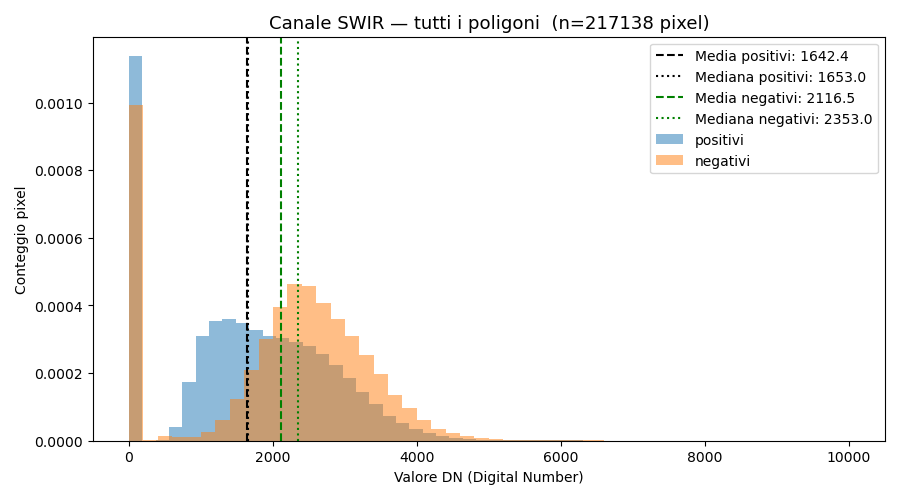
\includegraphics[width=0.9\textwidth]{capitoli/capitolo2/images/avocado/SatelliteSWIR.png}
    \end{minipage}
    \caption{Si mostrano i grafici infrarosso delle bbox degli avocado e dei non pianta}
    \label{fig:plotavocadoInfrarosso}
\end{figure}

Dato che alcuni valori (prossimi allo 0) rendono il grafico poco chiaro e difficile interpretare le differenze 
tra gli istogrammi, si è deciso di
rimuovere questi valori in modo da rendere il grafico interpretabile.

Come si evince dai grafici in quasi tutte le bande gli istogrammi sono quasi tutti sovrapposti. 
Si riesce a differenziare solo nelle 2 classi (avocado e non pianta) solo nelle bande dei grafici NIR e SWIR.
Questa separazione, sebbene non netta, indica che le bande infrarosse potrebbero essere le più informative 
per un ipotetico classificatore.

Si mostrano anche i bbox delle piante di tipologia 1 e 2 NIR prese dalle immagini fornite dall'azienda.

\begin{figure}[htbp]
    \centering
    \begin{minipage}{0.45\textwidth}
    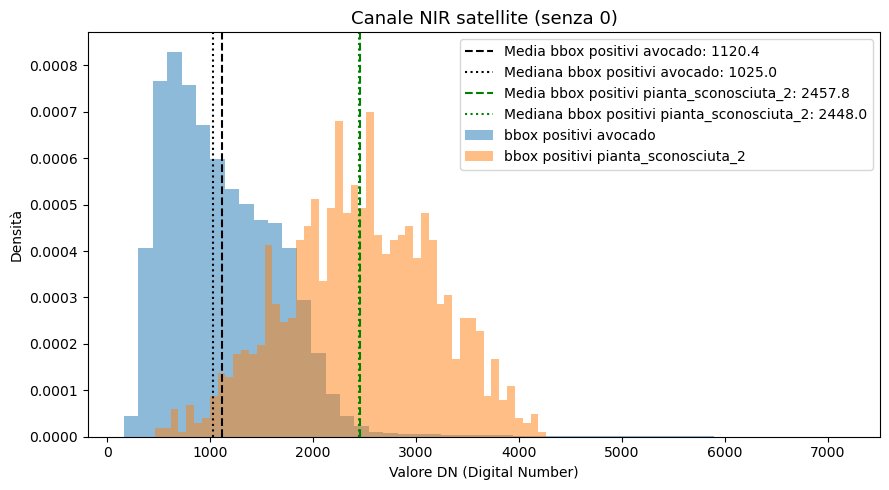
\includegraphics[width=0.9\textwidth]{capitoli/capitolo2/images/nir_pianta2_senza0.png}
    \end{minipage}
    \hfil 
    \begin{minipage}{0.45\textwidth}
    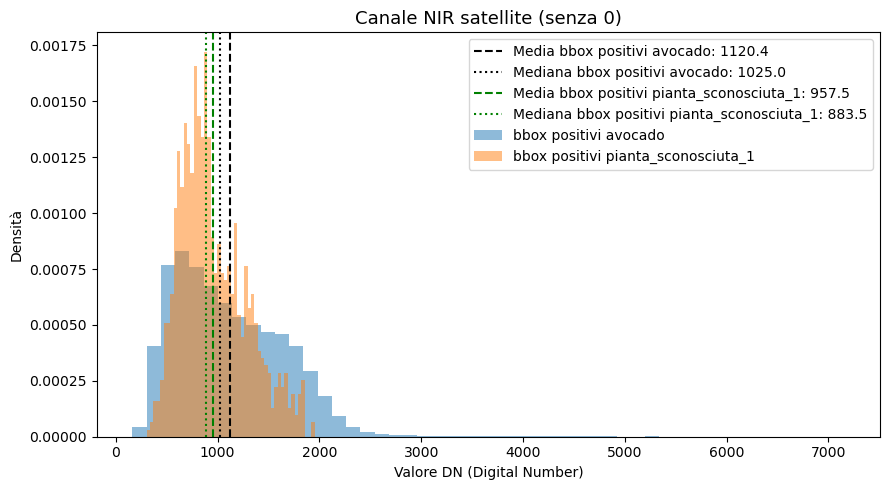
\includegraphics[width=0.9\textwidth]{capitoli/capitolo2/images/nir_pianta1_senza0.png}
    \end{minipage}
    \caption{Si mostrano i grafici NIR delle bbox delle tipologie di piante 1 e 2}
\end{figure}
\begin{figure}[htbp]
    \centering
    \begin{minipage}{0.45\textwidth}
    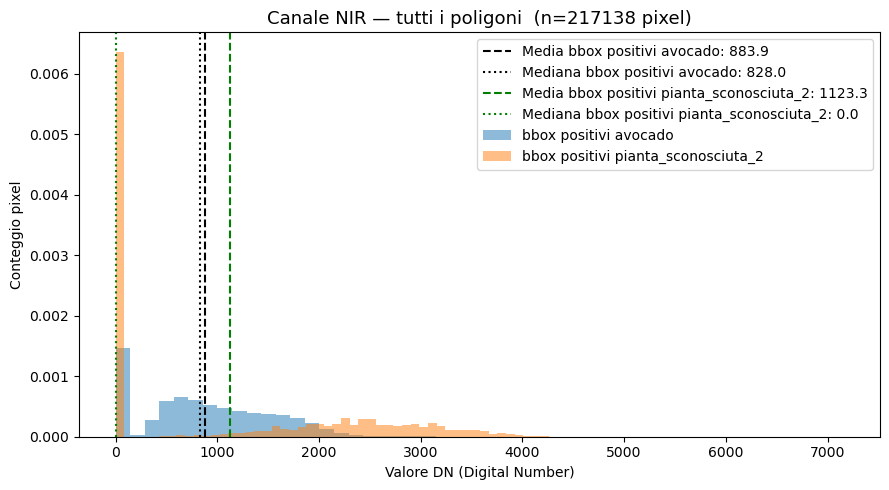
\includegraphics[width=0.9\textwidth]{capitoli/capitolo2/images/nir_pianta2.png}
    \end{minipage}
    \hfil 
    \begin{minipage}{0.45\textwidth}
    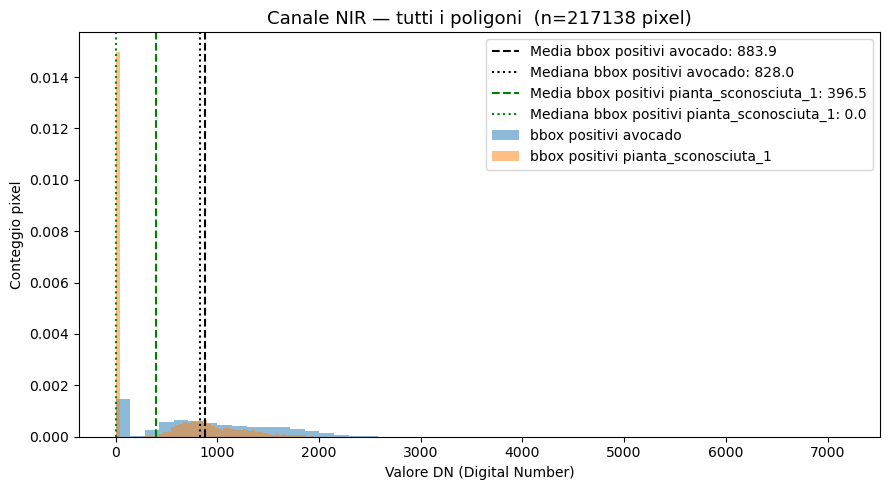
\includegraphics[width=0.9\textwidth]{capitoli/capitolo2/images/nir_pianta1.png}
    \end{minipage}
    \caption{Si mostrano i grafici NIR delle bbox delle tipologie di piante 1 e 2 togliendo i valori vicino allo 0}
\end{figure}

Ora si mostrano i grafici anche per il campo SWIR sempre per le stesse tipologie.

\begin{figure}[htbp]
    \centering
    \begin{minipage}{0.45\textwidth}
    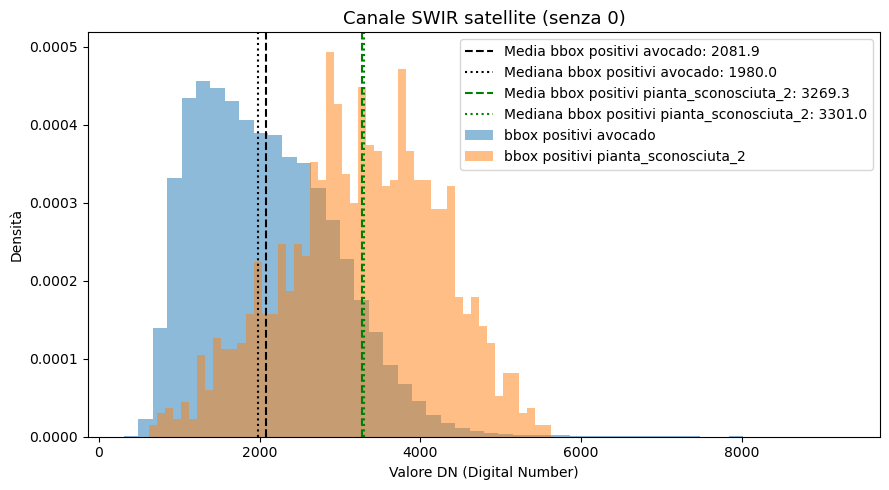
\includegraphics[width=0.9\textwidth]{capitoli/capitolo2/images/swir_pianta2_senza0.png}
    \end{minipage}
    \hfil 
    \begin{minipage}{0.45\textwidth}
    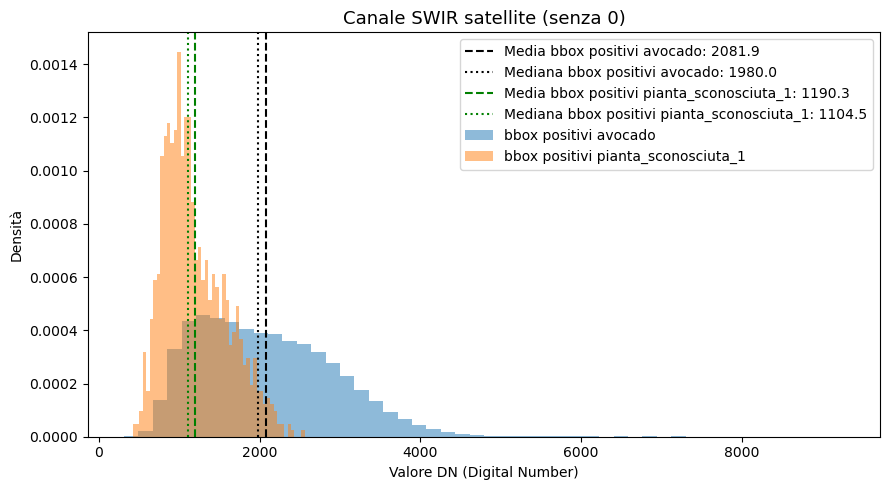
\includegraphics[width=0.9\textwidth]{capitoli/capitolo2/images/swir_pianta1_senza0.png}
    \end{minipage}
    \caption{Si mostrano i grafici SWIR delle bbox delle tipologie di piante 1 e 2}
\end{figure}
\begin{figure}[htbp]
    \centering
    \begin{minipage}{0.45\textwidth}
    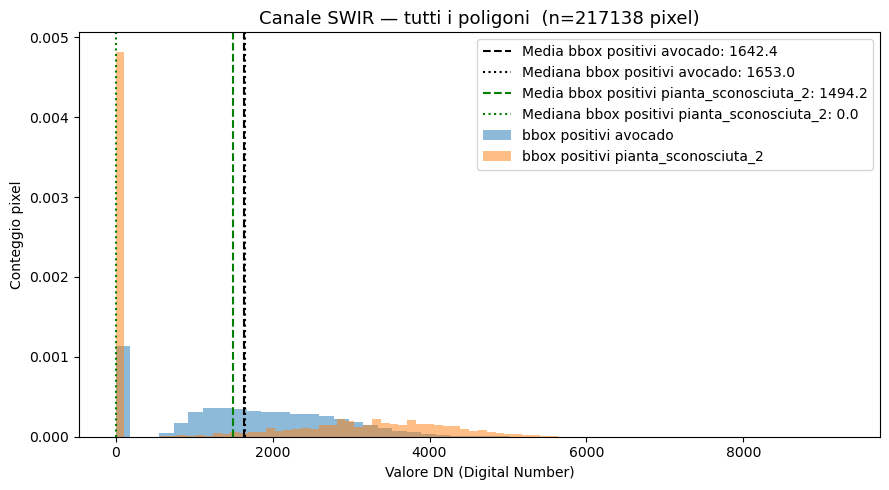
\includegraphics[width=0.9\textwidth]{capitoli/capitolo2/images/swir_pianta2.png}
    \end{minipage}
    \hfil 
    \begin{minipage}{0.45\textwidth}
    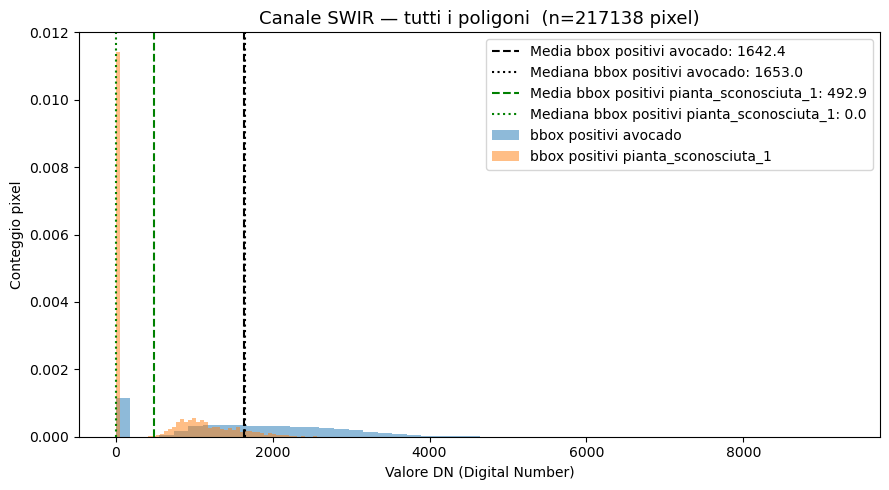
\includegraphics[width=0.9\textwidth]{capitoli/capitolo2/images/swir_pianta1.png}
    \end{minipage}
    \caption{Si mostrano i grafici SWIR delle bbox delle tipologie di piante 1 e 2 togliendo i valori vicino allo 0}
\end{figure}

Come si può osservare dai seguenti grafici tutte le tipologie 
di piante analizzate è possibile distinguere visivamente le distribuzioni di tutte le tipologie.

\section{Valutazione degli approcci possibili}

Per i classificatori si userà una Foresta Casuale \ref{subsec:foresta_casuale} per decidere, 
per ogni Pixel, se il pixel appartiene oppure no ad una pianta tipologia di pianta. 
Successivamente si andrà ad applicare una Regressione Lineare 
\ref{subsec:regressione_lineare} per comprendere il numero di piante dato il 
numero di pixel di una sagoma.



\section{Valutazione degli approcci possibili}

Si sa che il drone è un DJI Mavic 3 Multispectral. Ha volato con quota 14 m di altezza. 
La formula per trovare la risoluzione dei pixel è:
\[
GSD=\frac{H \cdot S_w}{f \cdot I_w}
\]
Dove $H$ è l'altezza in volo, $S_w$ è la larghezza del sensore, $f$ è la focale e $I_w$ è la larghezza immagine in pixel. Quindi la formula diventa:
\[
GSD=\frac{14m \cdot 17.3mm}{ 12mm \cdot 5280 px}=0.38 cm/px
\]
Di conseguenza:
\[ 
\text{ScaleFactor}=\frac{30cm/px}{0.38cm/px}=78.95
\]
